% File: algo.tex
% Date: Thu Jun 20 20:43:35 2013 +0800
% Author: Yuxin Wu <ppwwyyxxc@gmail.com>
\section{算法说明}
\subsection{光线追踪及光照模型}
光线追踪的基本原理如下图所示.
\begin{figure}[H]
  \centering
  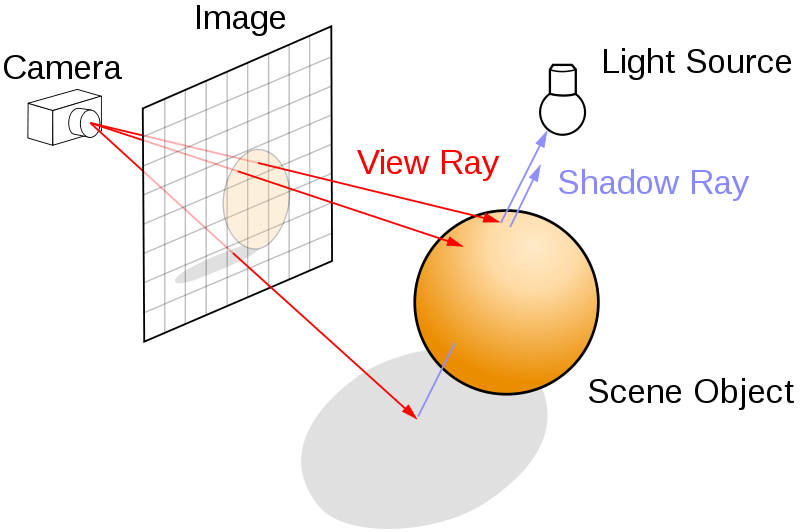
\includegraphics[scale=0.4]{res/ray_tracing.png}
\end{figure}

选定视点位置及一观察屏,从视点到屏上各点发出光线与空间中物体求交.
在交点处根据局部光照模型计算颜色,再递归的计算反射、透射光颜色,混合后显示在屏上.

此程序使用的局部光照模型为Phong模型,其主要公式为\cite{phong}:

\[  I_p = k_ai_a + \sum_{m\in lights} (k_d ( \overrightarrow{L_m} \cdot \overrightarrow{N} i_{m, d} + k_s(\overrightarrow{R_m}\cdot
  \overrightarrow{V})^{\alpha} i_{m, s}))  \]

其中$ k_s, k_d, k_a, \alpha$分别为物体表面该点处的高光系数,漫反射系数,环境光系数,亮度.
$ \overrightarrow{L_m}$为该点指向光源的向量, $ \overrightarrow{N}$为表面法向,
$ \overrightarrow{R_m}$为光源指向该点的光线经理想反射后的指向,
$ \overrightarrow{V}$为视点到表面交点处的向量.

\subsection{几何对象表示及计算}
程序支持了平面、球、三角面片、包围盒四类基本几何物体,
物体都需要各自拥有与光线求交的方法.

\begin{description}
  \item[光线]光线是一条射线,包含一个起始点及方向. 见\verb|include/geometry/ray.hh|
  \item[无穷平面]
    为了计算方便,使用平面法向及平面到原点的距离作为确定平面的方式.
    平面与光线求交时,首先通过光线指向判断是否相交,再通过
    光线在平面法向方向的投影长度计算交点.见\verb|include/geometry/infplane.hh, renderable/plane.cc|

  \item[球]球由球心及半径唯一确定.球与光线求交时,
    利用球心到它在光线所在直线上的投影的距离判断是否相交,在根据投影位置
    及勾股定理计算交点. 求交时要考虑光线起始点在球内部的情形.见\verb|include/geometry/sphere.hh, renderable/sphere.cc|

  \item[三角面片]三角面片用三个顶点坐标存储.
    为了性能,与光线的求交参考了\cite{triangle, triangle_code}的算法及实现,其基本思想是求解满足
    方程
    \[  \overrightarrow{Orig} + t * \overrightarrow{Dir} = x * \overrightarrow{v_1} + y  \overrightarrow{v_2} + (1 - x -
    y)\overrightarrow{v_3}, t > 0, x, y \in (0, 1), x + y \le 1\]
    的$ (t, x, y)$, 在求交时同时能得到交点的重心坐标\footnote{\url{https://en.wikipedia.org/wiki/Barycentric\_coordinate\_system}}
    ,便于之后进行法向插值.见\verb|include/renderable/face.hh, renderable/face.cc|

  \item[轴平行包围盒]
    轴平行包围盒用最小坐标与最大坐标两个向量存储.
    为了效率,包围盒与光线求交部分参考了\cite{aabb}的算法.
    其基本思想是对每个面逐一计算并更新交点.见\verb|geometry/aabb.hh|
\end{description}

\subsection{视图模型}
一个视图应包括视点及屏幕,且应使视点在屏幕的中轴线上.
视图类\verb|View|存储了视点坐标,屏幕中心坐标,屏幕尺寸,屏幕边沿的空间指向,
这样可以方便的进行视图旋转,视图平移,缩放等导航操作.见\verb|include/view.hh, view.cc|

\subsection{KD树}
KD树是一种空间划分树,原本用于在K维空间中快速查找点,可利用在光线追踪中对物体及其包围盒进行索引.
基本方法是,树中每个节点对应一个包围盒,选取一个轴平行平面将包围盒一分为二作为两个子节点,叶节点维护待存储的物体.
与切分面相交的物体在两节点中都应存储.

\subsubsection{建树}
传统的KD树中,按照使两边点的个数尽量接近的原则选取切分平面,这是由于假设了各个点被查询的概率均等.
在光线追踪中,一般采用面积启发式的平面选取方式\cite{kdtree},选取切平面使得
两个子节点的包围盒表面积与包含物体个数的积之和尽量大,这样可以使KD树在查询时效率更高.
但启发式的建树需要枚举切分平面,计算包含物体个数,复杂度较高.
直接的枚举为$ O(n^2)$复杂度,本程序实现了\cite{kdtree}中提供的$ O(n \log^2(n))$算法.
对于20W面片的龙模型\footnote{models/fixed.perfect.dragon.100K.0.07.obj},
采用不同方法单线程建树的用时及在几个固定视角渲染耗时如下(单位: 秒):

\begin{table}[H]
  \begin{threeparttable}

    \begin{tabular}{c|c|c|c|c|c|c}
      \shline
      & 建树 & 视角1 & 视角2 & 视角3 & 视角4 & 视角5 \\ \hline
      二分建树(终止:100层,15个)  & 0.6  & 1.93  & 2.51  & 3.26  & 4.38  & 5.89  \\ \hline
      SAH建树(终止:100层,20个) & 5.41 & 0.29  & 0.37  & 0.45  & 0.59  & 0.78    \\ \hline
      SAH建树(终止:100层,15个) & 7.82 & 0.24  & 0.33  & 0.41  & 0.52  & 0.68    \\ \shline
    \end{tabular}
    \begin{tablenotes}
      \footnotesize
    \item 注: 建树时,以树深度及当前节点所管理的物体个数作为建树结束的判定条件.
    \item 此实验的视角1为\verb|main.cc|中\verb|test_kdtree()|提供视角,其余视角由视角1 zoom in依次得到.
    \item 可在\verb|lib/kdtree.cc|中通过注释\verb|KDTree::build()|函数中相应代码切换两种建树算法.
    \end{tablenotes}
  \end{threeparttable}
\end{table}

由表可见SAH建树的查询效率有很大提高,但建树缓慢. 建树效率与渲染效率之间存在trade-off,可以通过改变终止条件来调整.

\subsubsection{求交}
求交的基本方法为,递归寻找两子树的最近\underline{物体}的交点,取较近者为结果返回.

实现时,在每个节点处保存了当前节点的两个孩子的切分平面,这样可以预先判断出离
光线较近的包围盒,若与其内物体相交则不用考虑另一包围盒.
此时应注意,若光线与第一个包围盒所管理的物体相交,应确认与最近物体的交点是否被第一个包围盒\underline{包含}.
因为若不包含,则光线首先打到的物体可能并不是此物体,而是第二个包围盒管理的物体.



\subsection{其他}
光线密度,折射
反射+EPS,
